\chapter{Einführung}
\section{Versionskontrolle}
Versionskontrollsysteme protokollieren Änderungen an Dateinen und ermöglichen es zu jedem Zeitpunkt auf eine ältere Version zuzugreifen.
\section{Git}
Im Gegensatz zu zentralen Versionskontrollsystemen handelt es sich bei Git um ein verteiltes Versionskontrollsystem (DVCS). Jeder Anwender clont das komplette Repository und erhält somit eine vollständige Kopie des Projektes.
\begin{figure}[ht]
	\centering
		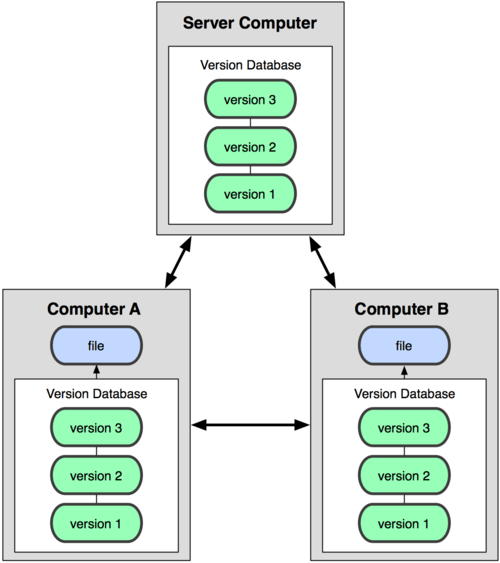
\includegraphics[width=0.5\textwidth]{img/dvcs.png}
	\caption{Verteilte Versionskontrolle}
\end{figure}
\subsection{Arbeitsweise}
Git speichert bei jedem Commit nur die geänderten Dateien. Nicht geänderte Dateien werden mit einem Verweis auf die alte Version übernommen. Es werden keine Informationen von anderen Rechnern im Netzwerk benötigt, da Git fast alle Operationen lokal ausführt und die Informationen ebenfalls in einer lokalen Datenbank hinterlegt werden. Änderungen werden zur Sicherstellung der Integrität mit Check\-summen überprüft.
\begin{figure}[ht]
	\centering
		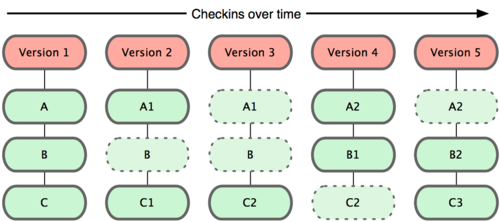
\includegraphics[width=0.6\textwidth]{img/snap.png}
	\caption{Git Snapshots}
\end{figure}
\subsection{3 Zustände}
Git definiert drei Hauptzustände, in denen sich eine Datei befinden kann. 
\begin{itemize}
\item \textbf{commited}\\
Daten sind in der lokalen Datenbank gesichert
\item \textbf{modified}\\
Datei wurde geändert, aber noch nicht commited
\item \textbf{staged}\\
Datei im gegenwärtigen Zustand für nächsten Commit vorgemerkt
\end{itemize}
\section{Git Config}
Git kann per Config Dateien angepasst werden. Der Befehl \texttt{git config} führt alle Optionen auf.
\section{Manpage}
Die Manpage hat den Vorteil, dass sie auch offline aufgerufen werden kann. Folgende Befehle stehen zur Auswahl:
\begin{lstlisting}[caption={Git Manpage},captionpos=b]
git help <verb>
git <verb> --help
man git-<verb>
\end{lstlisting}
